\documentclass[a4paper,german]{letter}

\usepackage{geometry}

\usepackage{german}
\usepackage{ngerman}
\renewcommand{\enclname}{Anlagen} %Anlagen statt Anlage(n)

\usepackage[utf8x]{inputenc}
\usepackage{hyperref}
\usepackage[left]{eurosym}
\usepackage{pdfpages}
\usepackage{fancyhdr}
\usepackage{color}
\usepackage[T1]{fontenc}
\newcommand{\hilight}[1]{\colorbox{yellow}{#1}}

\usepackage[babel,german=quotes]{csquotes} %\enquote{...} für deutsche Anführungszeichen um ein Wort
\usepackage{times}
% \setlength{\textwidth}{18cm}
% \setlength{\leftmargin}{-5cm}
% \setlength{\rightmargin}{0cm}
% \setlength{\evensidemargin}{0cm}
% \setlength{\oddsidemargin}{0cm}
%\input{hyphenation.tex}

\renewcommand{\headheight}{0.6in}
\renewcommand{\headrulewidth}{0.6pt}
\renewcommand{\footrulewidth}{0.6pt}
\setlength{\headwidth}{\textwidth}

\fancyhead[R]{\includegraphics[height=0.3in]{../vorlagen/logo.pdf}} % Aus unklaren Gründen geht hier kein cm als Einheit!
% \fancyhead[L]{\hilight{ENTWURF}}
% \fancyfoot[L]{\hilight{ENTWURF}}
% \fancyfoot[R]{Stand \today}
\pagestyle{fancy}

\address{FAU FabLab\\Lehrstuhl 3 der Informatik\\Martensstraße 3\\91058 Erlangen}
\signature{FAU FabLab}
\begin{document}
\begin{letter}{Dr.-Ing. Jochen Weinzierl\\ Geschäftsstelle EEI\\ Cauerstr. 7\\ 91058 Erlangen}
\thispagestyle{fancy}
\bigskip
\fancyhead[R]{\includegraphics[height=0.3in]{../vorlagen/logo.pdf}}
\opening{Betrifft: Aufrüstung der Räume des ehemaligen Netzmodells zur Nutzung durch FSV und FabLab}
\smallskip

\thispagestyle{fancy} %nötiger Fix, damit auch die erste Seite die Kopf- und Fußzeile verpasst bekommt
Sehr geehrter Herr Dr. Weinzierl,

nach dem Auszug des Netzmodells aus den Räumen U1.237-U1.239 im MHB-Gebäude sollen die Räume U1.239 und U1.238 durch das FabLab sowie Raum U1.240 von FSV und FabLab gemeinsam genutzt werden. % Dieser Satz ist scheiße
Damit die Räume zum größtmöglichen Nutzen der Studierenden eingesetzt werden können, haben wir Pläne erstellt, was für einen sinnvollen Betrieb des FabLabs notwendig ist. Daraus ergeben sich einzelne Baumaßnahmen sowie Anschaffungskosten für das Mobiliar, sofern wir dieses nicht anderweitig kostenlos beschaffen können.

Wir bitten Sie darum, diese Anforderungen mit einzubeziehen und uns an der weiteren Planung mit zu beteiligen. Im Vergleich zu den Gesamtkosten werden diese Punkte eine überschaubare Summe sein, sodass sie aus den Mitteln des Antrags \enquote{Räume für Studierende im MHB-Gebäude} mitfinanziert werden sollen.

Zum einen wird Infrastruktur benötigt, die (nach unserer jetzigen Kenntnis) bereits vorhanden ist. Dies sind unter anderem folgende Punkte:
\begin{itemize}
  \item Wasser- und Abwasseranschluss
  \item Fliesenboden in einem Raumteil
  \item breite Doppeltüre
  \item Doppelboden im anderen Raumteil
  \item Druckluftanschluss (optional, nur wenn wirklich bereits vorhanden und machbar)
  \item Licht (ausreichend hell zum Arbeiten, in vernünftigem Zustand)
  \item Telefon (mit Amtsberechtigung zum Festnetz außerorts, Abrechnung z.B. auf Informatik LS 3)
  \item Wand zwischen Doppelboden- und Werkstatt-Raum: Diese soll nach jetziger Raumplanung \emph{nicht} enfernt werden, weil dort Regale stehen sollen.
\end{itemize}

Diese Punkte sollen bei den Baumaßnahmen auf jeden Fall erhalten bleiben oder, falls nicht mehr vorhanden, wieder neu geschaffen werden.

\newpage
Um einen vernünftigen Betrieb des FabLabs zu ermöglichen, ist zusätzlich die folgende Infrastruktur erforderlich:
\begin{itemize}

\item Benutzung 24/7 möglich: Rund um die Uhr, auch feiertags und am Wochenende
	\begin{itemize}
	\item Benutzungsmöglichkeit und Zugang (per FAU-Card) von außen bis in die Räumlichkeiten.
	\item Zugangsberechtigungen unbürokratisch änderbar, Liste der Leute mit Zugang und Gültigkeitsdauer wird durch FabLab bzw. FSV festgelegt.\\
	\end{itemize}


\textbf{offene Punkte:} Außenzugang schon vorhanden? Finanzierung?
\item Einbau einer Türe zwischen U1.240 (Besprechungsraum FSV/FabLab) und U1.239 (FabLab), die von U1.239 aus per Klinke geöffnet werden kann, von U1.240 aber nicht (oder nur mit Schlüssel) geöffnet werden kann. \\ \textbf{offener Punkt:} Die genaue Position der Türe muss noch abgestimmt werden, da wahrscheinlich Leitungen in der Wand verlaufen.
\item Einbau von Siport Schließanlagen an die Außentüren von U1.240 und U1.239\\
\textbf{offener Punkt:}  Finanzierung (über anderen Studiengebühren-Antrag \enquote{Schließanlagen}?)
%\item \hilight{noch offen: Entweder Kartenleser an beiden Außentüren, oder Kartenleser an Außentüre} \\\hilight{ U1.240 und die Zwischentüre von dort nach U1.239}

\item ausreichend Strom
	\begin{itemize}
	\item Hauptsicherung >= 35A (besser 63A)
	\item Hauptsicherung selektiv zur übergeordneten Sicherung: Die übergeordnete Sicherung löst noch nicht aus, wenn die Hauptsicherung auslöst
	\item Sicherungen (auch Hauptsicherung) und FI-Schutzschalter im Raum zugänglich, ausgeführt als Sicherungsautomaten (keine Schmelzsicherungen)
	\item 3 voneinander getrennt abgesicherte Drehstromsteckdosen CEE 16A% (Fräse, Bohrmaschine, Abluftanlage)
	\item je Raum 3 voneinander getrennt abgesicherte Steckdosen-Stromkreise, je 16A, mit FI-Schutzschalter% (Werkstatt: Lasercutter+Lüftung, Werkstattgeräte, Computer; Elektrolabor: Laborgeräte, Computer, Reserve)
	\item ausreichende Anzahl von Steckdosen in beiden Räumen (Werkstatt: an der Wand, Elektrolabor: möglichst im Doppelboden)
	\end{itemize}

\item Netzwerk: LAN Gigabit, Verbindung ins FabLab-Netz der Informatik % Gigabit wegen Anbindung an Fileserver
\item im Werkstattraum (U1.239):
	\begin{itemize}
	\item Abluftauslass (Loch durch die Wand, wie für Dunstabzugshaube) mit Durchmesser $\geq$ 110mm für Lasercutter- und Fräsen-Abluft (nur Loch mit Rohr und äußerer Abdeckung nötig, der Rest innen im Raum wird vom FabLab selbst eingerichtet)
	\item Durchlass für Kabel zum anderen Raum, z.B. ein größeres Loch durch die Wand auf Bodenhöhe, sodass es innerhalb des Doppelbodens endet
	\end{itemize}


\item Mobiliar (ein Teil davon kann evtl. durch Spenden aus der Informatik abgedeckt werden):
	\begin{itemize}
	\item 7 Tische etwa 80x160cm, möglichst mit Durchführungen für Kabel
	\item 1 Whiteboard etwa 1x2m (evtl in der Informatik übrig)
	\item 2 Werkbänke oder ähnlich solide Tische (vermutlich Spende vom LS Informatik 3)
	\item 14 Stühle, größtenteils mit Rollen, halbwegs bequem (keine alten Holzhocker)
	\item 1 stabile Trittleiter
	\item 5 besonders belastbare Regale: Schäfer FIX-Schraubregal verzinkt Profil 2 \\
		HxBxT 192x100x60cm mit 5 Böden, Art.Nr. 31119-SW21 (260€/Stk inkl. MwSt.), oder Vergleichbares (1 weiteres ist bereits vorhanden)
	\item Neues Waschbecken: Aus Keramik (kein Stahl/Edelstahl!), ausreichend tief (für Keller/Werkstatt gedachte Modelle, Hahn weiter oben an der Wand montiert). Bisher ist scheinbar nur ein schmaler Wasserablaufschlitz, aber kein anständiges Becken vorhanden.
	\item eventuell: Holzplatten, Balken, Winkel und Schrauben für einzelne Eigenbautische (wenn sich bei den als Sondermaß eingezeichneten Tischen nichts passendes als Spende aus der Informatik findet)
	\item Löcher bohren und Dübel setzen zur Befestigung von Regalen und sonstigem Mobiliar (muss wahrscheinlich über ATD erfolgen, Kosten unklar)
	\item lange Netzwerkkabel, Switche, USB-Hubs und -Verlängerungen für Geräte (teilweise Spenden aus der Informatik)
	\item diverser Kleinkram
	\end{itemize}
\end{itemize}

Wir bemühen uns, möglichst viele Punkte davon kostenlos umzusetzen. Wo dies jedoch nicht möglich ist, bitten wir Sie darum, die entsprechenden Punkte zu finanzieren.

Bei Nachfragen und neuen Informationen können Sie sich gerne an mich wenden. Ebenso werden wir Sie informieren, sobald sich offene Punkte geklärt haben.

% Optional:
% \item Zugang direkt von Außen durch eine zusätzliche Tür, befahrbar für Hubwagen
% \item Schallgedämmte Wand richtung Hörsääle
% \item Maschinenbett für Fräse
% \item Werkbänke (wo auch die Standbohrmaschine stehen soll)

 %\closing{Mit herzlichen Gr"u"sen}
\vspace{1em}
Mit freundlichen Grüßen

\includegraphics{/home/max/privat/unterschrift.pdf}

Max Gaukler\\
FAU FabLab

Email: max@fablab.fau.de

\vspace{1em}

 \encl{Übersichtsplan\\Raumplan}
\end{letter}
\newpage
\thispagestyle{empty}
\hspace{-1.5cm}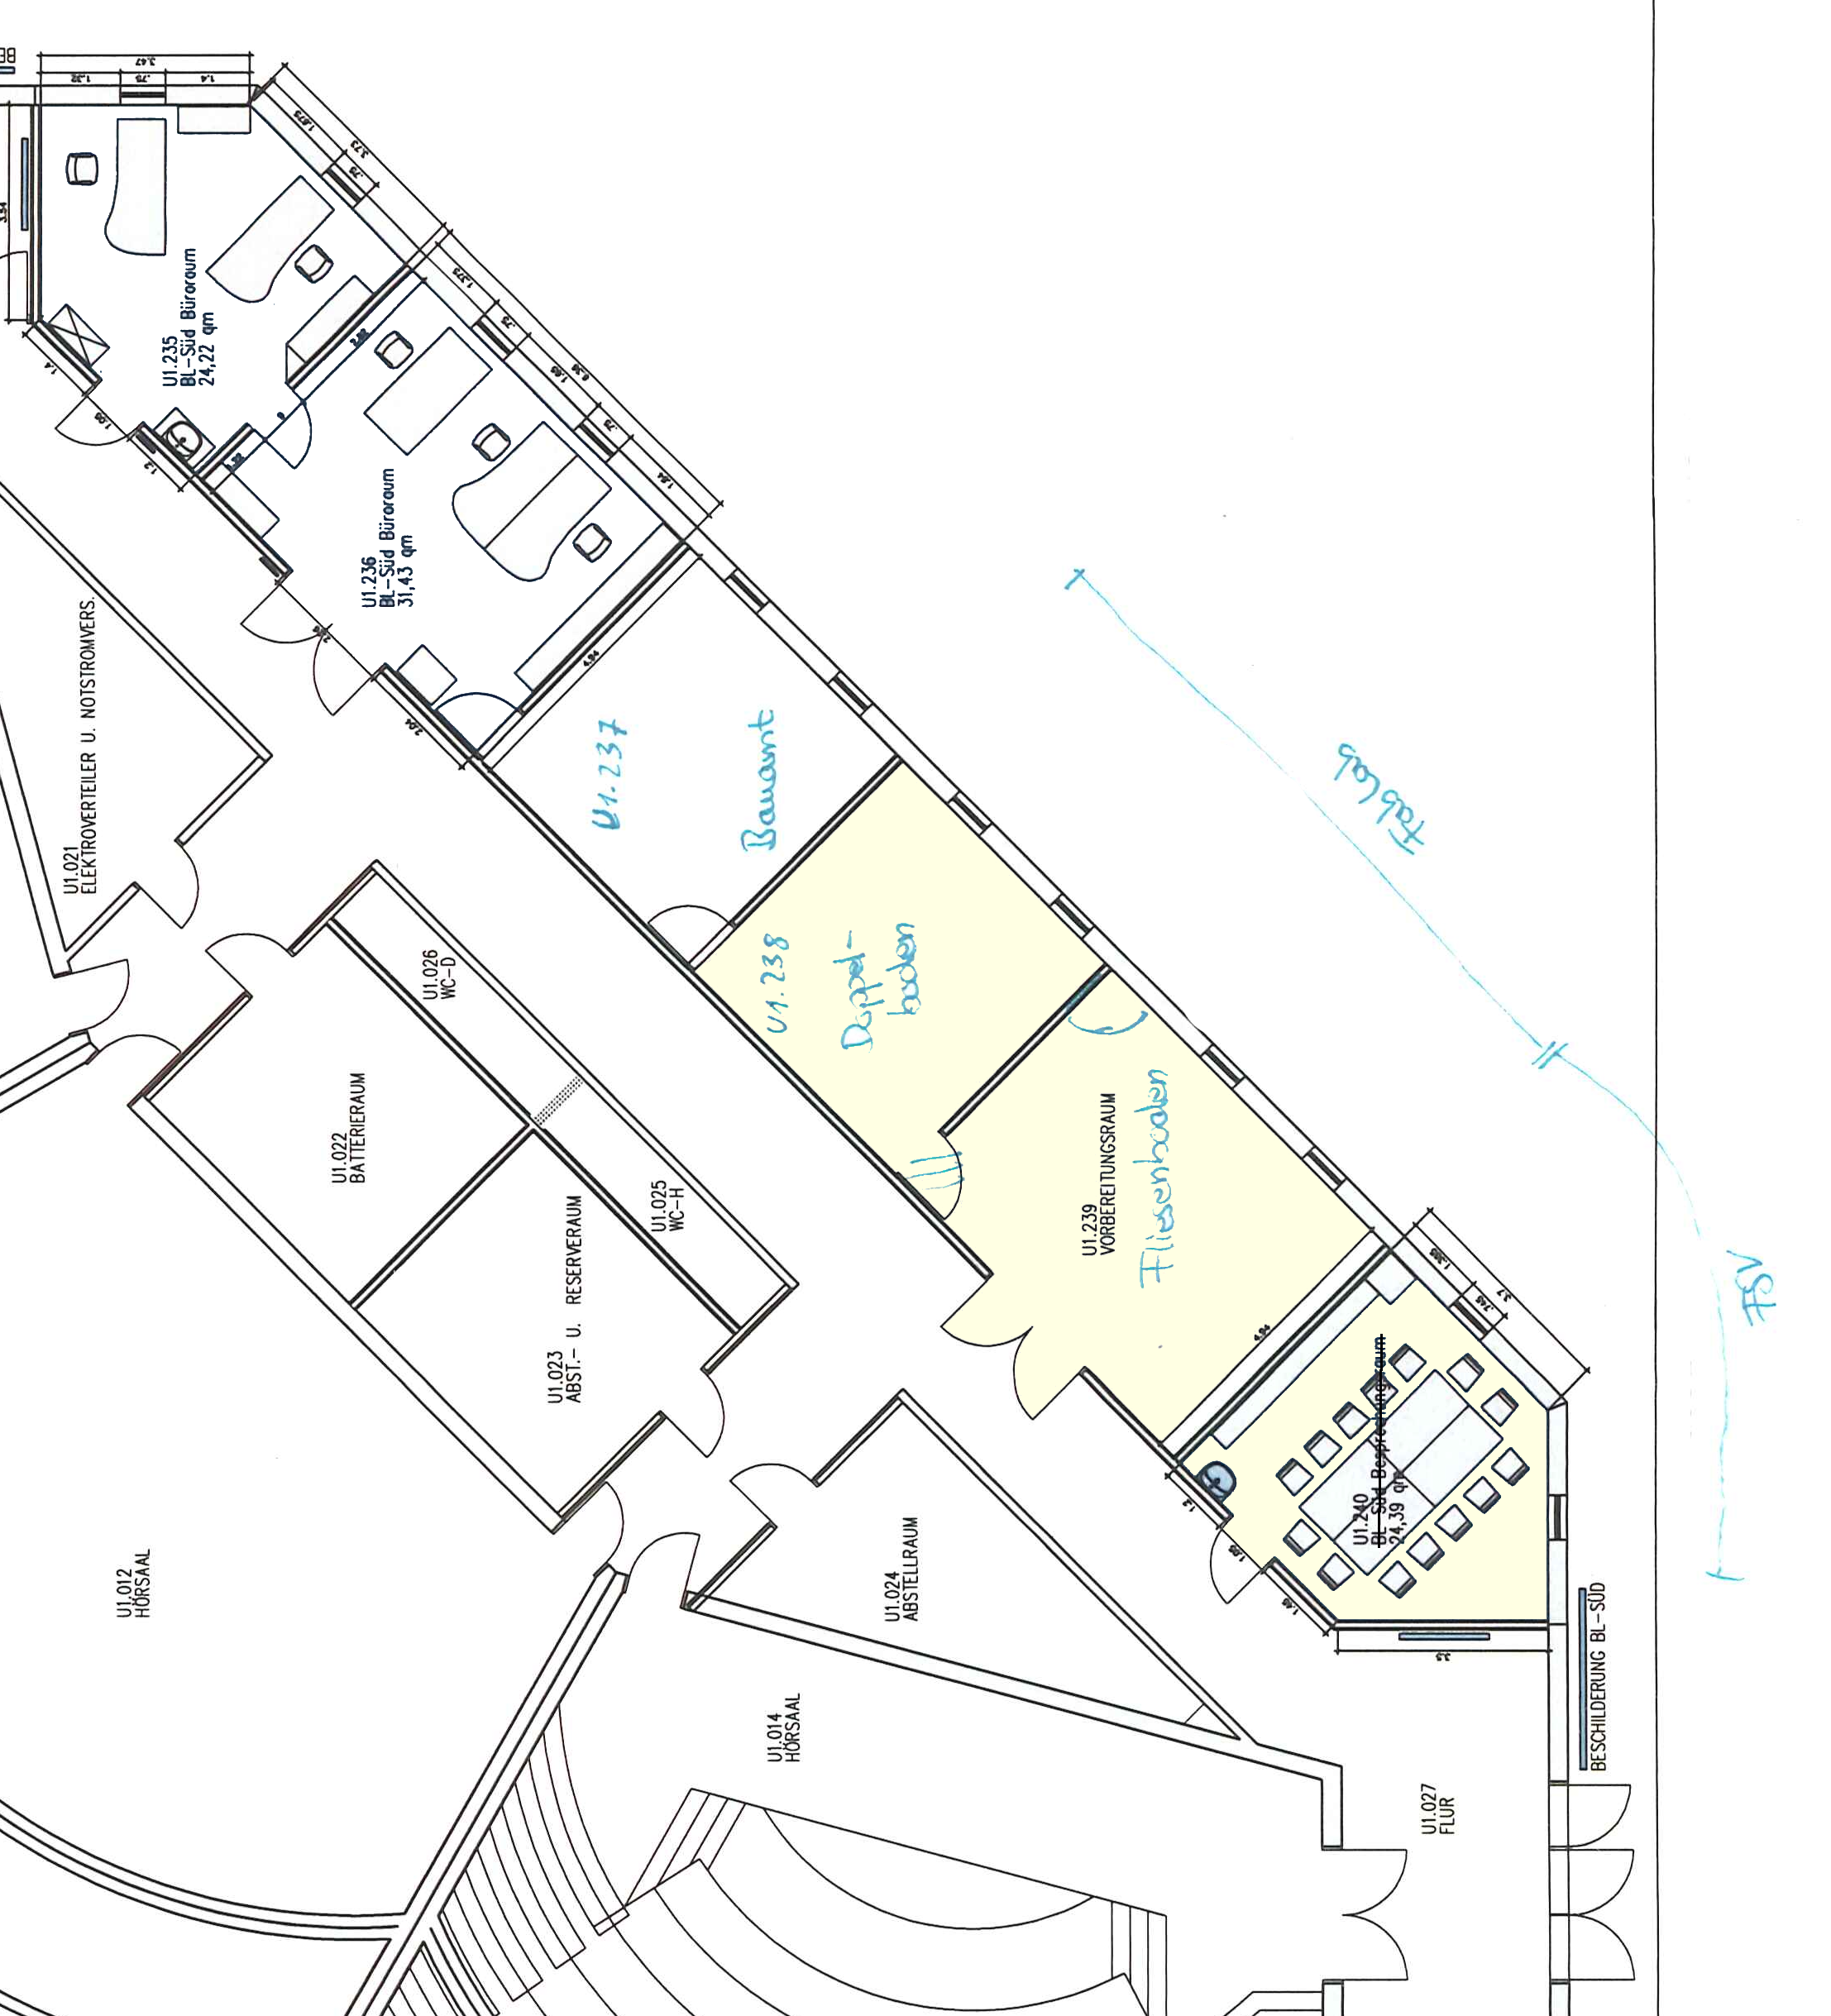
\includegraphics[width=18cm]{./mhb-raumplan-ausschnitt.png}
\includepdf[pages=-]{./mhb.pdf}
\end{document}